\section{The price field as an assignment equilibrium}
\label{sec:microfoundation}

The price field $\Pi(r)$ enters the model as a reduced form: it is the
capability-price surface estimated in \textcite{storck2026geometry}, taken as
given. This section asks whether it can instead be \emph{derived} as the
equilibrium of a closed model, and uses a sequence of tests to select the
closure. The exercise is reproducible in \texttt{scripts/12\_price\_microfoundation.py};
the numbers below are its output. The conclusion is that $\Pi(r)$ is neither a
task-scarcity nor a factor-scarcity object but the equilibrium price of a
multidimensional capability \emph{assignment} with cognitively biased demand,
and that this closure derives the directed gradient rather than assuming it.

\paragraph{Scarcity is the wrong margin.}
The simplest closure is a CES aggregator over tasks,
$Y = \big[\int_{D} \alpha(r)\, y(r)^{(\sigma-1)/\sigma}\, dr\big]^{\sigma/(\sigma-1)}$,
whose first-order condition prices each task at
$p(r) = \alpha(r)\,(Y/y(r))^{1/\sigma}$: high where the task is demanded
($\alpha$ large) and scarce ($y$ small). With $\alpha$ uniform and task output
proportional to the labour serving it, $\ln\Pi(r) = \text{const} - \sigma^{-1}\ln
n_0(r)$, so the price should fall with employment density. It does not: the
fitted slope is $-0.03$ (an implausible $\sigma \approx 35$), and the dear
socio-cognitive north is in fact \emph{more} densely staffed than the cheap
south (log-density difference $+0.71$). The directed gradient is not a
task-scarcity phenomenon.

\paragraph{The field is a hedonic capability surface.}
What the price does track is capability content. The log price is $96$ percent
linear in the capability-weighted requirement $\sum_k v_k q_k(r)$
($R^2 = 0.956$), dominated by the cognitive capability $S_1$
($v_{S_1} = +0.33$, against near-zero weights on the others). This is exactly
the finding of \textcite{storck2026geometry} that markets price capabilities
rather than task depth, and it is the reason the reduced form is not atheoretic.
But the $v_k$ are not equilibrium factor prices: across the four capabilities the
price is \emph{negatively} related to scarcity ($\mathrm{corr}(v_k, 1/X_k) =
-0.28$, with $X_k$ the aggregate capability endowment), and one coefficient is
negative ($v_{A_1} = -0.03$). A competitively priced factor cannot have a
negative price; the $v_k$ are hedonic partial coefficients. A surface of hedonic
capability prices with a negative loading is the signature of multidimensional
sorting, not of a factor market, and it is sorting that the closure must
supply.\footnote{The $R^2 = 0.956$ is in part mechanical, since the price field
is itself constructed in capability terms; the substantive test is not that
$\sum_k v_k q_k$ fits $\Pi$ but whether the $v_k$ are equilibrium objects, which
the scarcity test rejects.}

\paragraph{The assignment closure.}
Let workers be the occupations, each a mass $L_o$ of capability type $\theta_o$,
with productivity at task $r$ given by the readiness $f(\theta_o,r) = e_o(r)$
(eq.~\ref{eq:readiness}). Final demand is CES over tasks with weight $\alpha(r)$.
A competitive equilibrium is a task price $\Pi(r)$, an allocation in which each
occupation sends labour to the tasks paying $\Pi(r) f(\theta_o,r)$ most, and a
wage $w_o$ that occupations earn, such that task markets clear. $\Pi(r)$ is the
dual of this assignment; the hedonic wage surface of Paper~1 is its shadow. We
solve the fixed point numerically (logit allocation at smoothness $\kappa$,
$\sigma = 3$), taking \emph{no} observed wages as inputs --- only the capability
distribution $G(\theta)$, the requirements $q(r)$, and demand $\alpha$.

\paragraph{The assignment derives the shape; demand derives the gradient.}
With uniform demand the equilibrium price reproduces the reduced-form field at
Spearman $0.91$ --- a wage-independent recovery of its \emph{shape}, robust to
$\kappa$ ($0.90$--$0.92$) and $\sigma$. But the directed gradient it produces is
roughly four times too flat (north$-$south $+0.08$ against the observed $+0.39$):
capability-constrained supply makes the north dear only weakly, and it predicts
the north \emph{scarce}, contradicting the data. Both gaps close under a single
cognitively biased demand parameter, $\alpha(r) = \exp(\lambda\, q_{S_1}(r))$. At
$\lambda \approx 0.2$--$0.25$ the equilibrium brackets the observed gradient
(north$-$south $+0.36$ to $+0.43$), turns the north abundant in sign, and lifts
the overall fit to its peak of Spearman $0.97$ (Figure~\ref{fig:price-microfoundation}).
The directed gradient is thus \emph{derived} as the equilibrium price of
cognitively intensive tasks under cognitively biased demand --- the
multidimensional analogue of the task-demand schedule that carries the wage
structure in \textcite{acemoglu2022tasks}.

\paragraph{It is demand, not productivity.}
A natural alternative would route the gradient through production: let
high-$S_1$ workers be especially productive at deep cognitive tasks, a
capability-task complementarity. This is rejected. Complementarity does
concentrate employment strongly in the north (north$-$south up to $+0.61$,
near the observed $+0.71$), but it \emph{crashes} wages there: the concentrated,
highly productive labour floods task output, and the CES price falls faster than
productivity rises, so northern wages drop \emph{below} southern (north$-$south
wage $-0.76$ to $-1.99$, against the observed $+0.46$). Productivity
complementarity yields an abundant-but-cheap north, the opposite of the data. The
dearness of cognitive work is therefore a demand phenomenon, not a production
one --- a conclusion the microfoundation reaches independently of, and in
agreement with, the reduced-form evidence.

\paragraph{What remains.}
One residual is honest and informative. The demand closure matches the
\emph{sign} of the north's employment concentration but understates its
\emph{magnitude} (model $\approx +0.05$ against the observed $+0.71$): the
$\lambda$ that fits the price gradient pulls in only modestly more labour than
uniform demand, and the $\lambda$ that would match the strong observed
concentration overshoots the price. A single log-linear demand shifter cannot hit
both magnitudes, and productivity complementarity --- the obvious second
instrument --- is ruled out by the wage evidence. The remaining concentration is
left to a richer demand structure (non-homothetic preferences, or a lower
inter-task elasticity), not to the production side. We therefore report the
price field as microfoundable in \emph{shape} (wage-independent, Spearman
$0.91$) and in \emph{directed gradient} (a single demand parameter, Spearman
$0.97$), with the magnitude of the employment concentration as a stated open
question. The microfoundation thus does more than fit: it decomposes $\Pi$ into a
capability-assignment cost envelope and a demand-driven cognitive premium, and
eliminates the scarcity and productivity accounts. This places the construction
at the intersection of the task-based tradition
\parencite{acemoglu2018race,acemoglu2022tasks} and multidimensional sorting
\parencite{lindenlaub2017,lisepostelvinay2020}, and answers the standing
objection that $\Pi$ is merely reduced form.

\begin{figure}[!htbp]
\centering
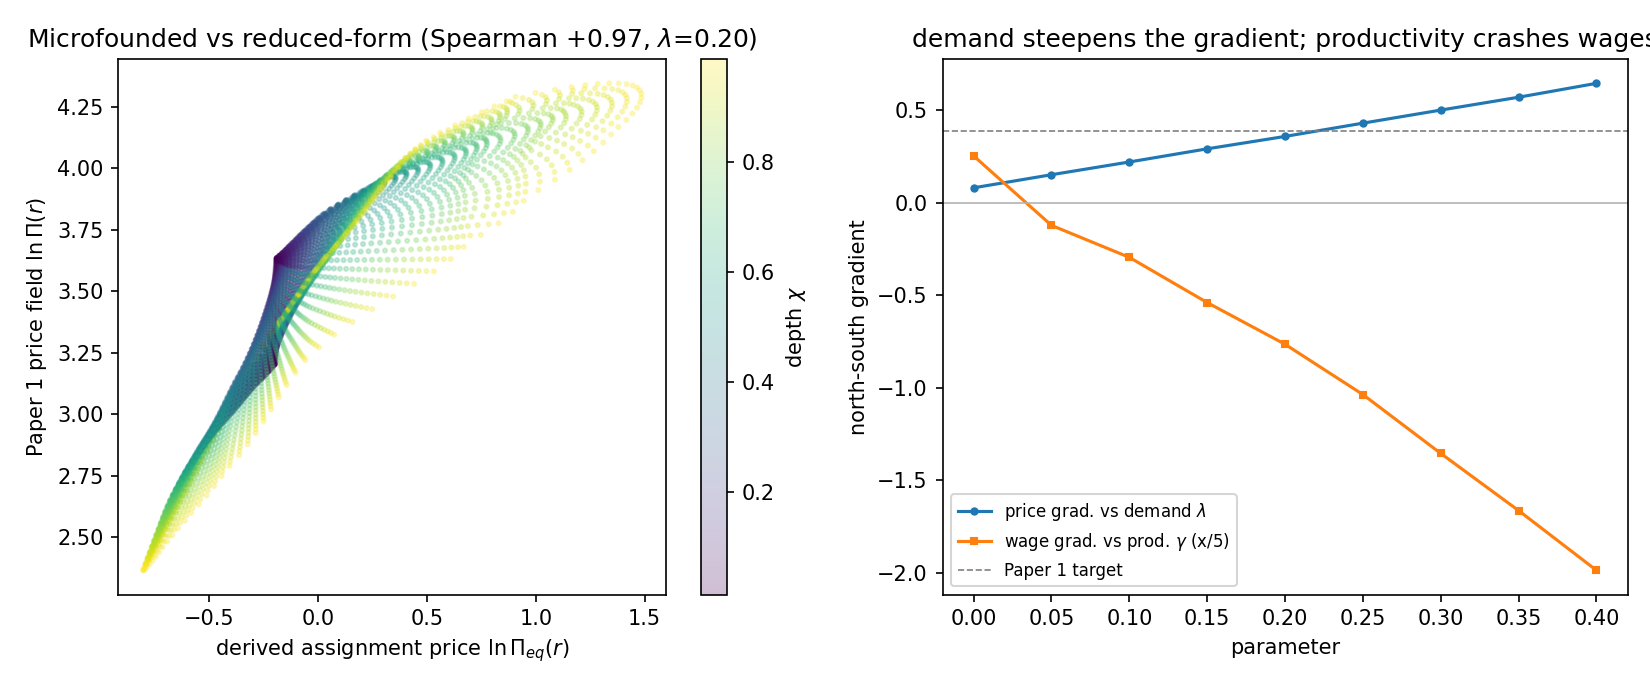
\includegraphics[width=\textwidth]{price_microfoundation.png}
\caption{\emph{Left:} the derived assignment price $\ln\Pi_{eq}(r)$ at the
calibrated demand bias against the reduced-form field $\ln\Pi(r)$, coloured by
task depth $\chi$ (Spearman $0.97$). \emph{Right:} the directed north$-$south
gradient as a function of the cognitive demand bias $\lambda$ (price) and the
productivity complementarity $\gamma$ (wage). Demand steepens the price gradient
to the Paper~1 target (dashed); productivity complementarity drives the wage
gradient \emph{negative}, an abundant-but-cheap north, and is rejected.}
\label{fig:price-microfoundation}
\end{figure}